\documentclass{article}

\usepackage[margin=1in]{geometry}
\usepackage{graphicx}
\usepackage{siunitx}
\usepackage{amsmath}
\usepackage{booktabs}
\usepackage{multirow}
\usepackage{caption}
\usepackage{array}
\usepackage[hidelinks]{hyperref}
\usepackage{indentfirst}
\usepackage{float}
\usepackage{enumitem}
\usepackage{xcolor}
\usepackage[numbers,sort&compress]{natbib}
\usepackage{tikz}
\usetikzlibrary{arrows.meta,positioning}

\newcommand{\maybeimage}[2][\textwidth]{%
  \IfFileExists{#2}{%
    \includegraphics[width=#1]{#2}%
  }{%
    \fbox{\parbox[c][0.22\textheight][c]{0.95#1}{\centering Missing image file: \texttt{#2}}}%
  }%
}

\title{RL vs PID for Adaptive Cruise Control\\
\large with different driving styles}
\author{Ruby Zhou}
\date{}

\begin{document}

\maketitle

\section{Introduction} Since I got rear ended yesterday, I thought it would be fun to do a report on adaptive cruise control. Adaptive cruise control is a driver-assistance system where a vehicle automatically adjusts its acceleration and braking to maintain a safe distance behind another vehicle. Basically, it follows the car in front of it in a safe and efficient way. However, unlike regular cruise control, which only tries to maintain a target speed, adaptive cruise control responds to changes in the speed of the lead vehicle, such as braking and acceleration. In this project, I simulate a simplified adaptive cruise control problem with two cars moving in one dimension. The \textbf{lead car} follows a scripted speed pattern, while the \textbf{ego car} is controlled by either a PID controller or a reinforcement learning policy. The ego car's goal is to follow the lead car safely and smoothly while maintaining a desired following distance. The main question I'm asking is: \begin{quote} Can a reinforcement learning policy learn adaptive cruise control behaviour comparable to a tuned PID controller? \end{quote} 

I also looked at a few research papers to see how other people approached this problem. Lin et al.\ compared deep reinforcement learning with model predictive control for adaptive cruise control, and they also treated acceleration as a continuous action \cite{lin2020comparison}. SAINT-ACC treats adaptive cruise control as a balance between safety, comfort, and traffic efficiency instead of only trying to minimize distance error \cite{das2021saint}. I also found research on personalized adaptive cruise control, where different cost functions are used to represent different driver preferences \cite{ozkan2021personalized}. This was useful for the driving style part of my project.

The main things I ended up investigating were:
\begin{itemize}
    \item how much tuning changes the PID baseline;
    \item how the reward function changes what PPO actually learns;
    \item why some random seeds converge while other seeds completely fail;
    \item whether the policy generalizes to lead-car behaviour it did not train on; and
    \item how the same ACC setup can produce aggressive, safe, or smooth behaviour.
\end{itemize}



\section{Related Work}

\subsection*{Classical vs. Learning-Based ACC}

Traditional adaptive cruise control normally uses feedback control or model predictive control. The nice thing about these methods is that they are easier to understand and much cheaper to run than a neural network. Deep reinforcement learning is different because it learns a policy from experience instead of being directly told a control equation.

Lin et al.\ used DDPG for adaptive cruise control and compared it against MPC \cite{lin2020comparison}. Their setup was especially relevant to mine because the action was also continuous acceleration, and the controller had to balance tracking, comfort, and control effort. SAINT-ACC also treats ACC as a multi-objective problem instead of only caring about distance error \cite{das2021saint}.

\subsection*{Why Multiple Seeds Matter}

A big issue with deep RL is that the exact same setup can give different results depending on the random seed. The neural network starts with different random weights, the environment samples different experiences, and the training path can end up somewhere completely different. Henderson et al.\ explain why reporting only one lucky run can make an RL method look much more reliable than it actually is \cite{henderson2018matters}. This is why I started using five-seed sweeps instead of only training one model.

\section{Simulator Setup}

The simulator contains two vehicles: the lead car and the ego car. Both cars move along a straight one-dimensional road. Each car has a position, speed, and acceleration.

\begin{figure}[h]
\centering
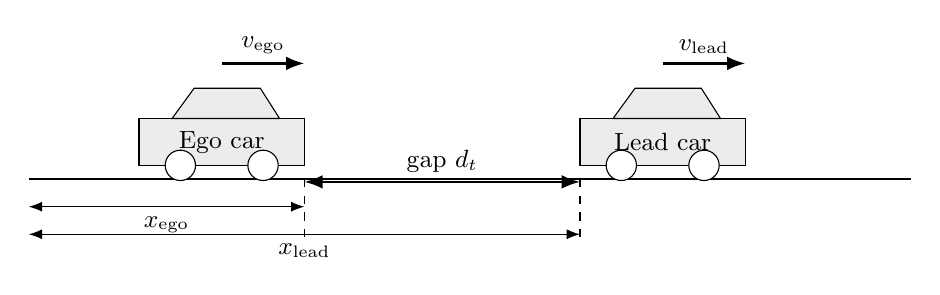
\begin{tikzpicture}[x=0.35cm,y=0.35cm,>=Latex]

% Road
\draw[thick] (0,0) -- (32,0);

% Ego car
\draw[fill=gray!15] (4,0.5) rectangle (10,2.2);
\draw[fill=gray!15] (5.2,2.2) -- (6.0,3.3) -- (8.4,3.3) -- (9.1,2.2) -- cycle;
\draw[fill=white] (5.5,0.5) circle (0.55);
\draw[fill=white] (8.5,0.5) circle (0.55);
\node at (7,1.35) {\small Ego car};

% Lead car
\draw[fill=gray!15] (20,0.5) rectangle (26,2.2);
\draw[fill=gray!15] (21.2,2.2) -- (22.0,3.3) -- (24.4,3.3) -- (25.1,2.2) -- cycle;
\draw[fill=white] (21.5,0.5) circle (0.55);
\draw[fill=white] (24.5,0.5) circle (0.55);
\node at (23,1.35) {\small Lead car};

% Velocity arrows
\draw[->, thick] (7,4.2) -- (10,4.2);
\node[above] at (8.5,4.2) {\small $v_{\mathrm{ego}}$};

\draw[->, thick] (23,4.2) -- (26,4.2);
\node[above] at (24.5,4.2) {\small $v_{\mathrm{lead}}$};

% Position markers
\draw[dashed] (10,0) -- (10,-2.2);
\draw[dashed] (20,0) -- (20,-2.2);

\draw[<->] (0,-1.0) -- (10,-1.0);
\node[below] at (5,-1.0) {\small $x_{\mathrm{ego}}$};

\draw[<->] (0,-2.0) -- (20,-2.0);
\node[below] at (10,-2.0) {\small $x_{\mathrm{lead}}$};

% Gap arrow
\draw[<->, thick] (10,-0.1) -- (20,-0.1);
\node[above] at (15,-0.1) {\small gap $d_t$};

\end{tikzpicture}
\caption{Schema of the 1D ACC simulator.}
\label{fig:acc_schematic}
\end{figure}

The basic vehicle dynamics are:

\begin{align}
v_{t+1} &= v_t + a_t \Delta t \\
x_{t+1} &= x_t + v_{t+1} \Delta t
\end{align}

where $x$ is position, $v$ is velocity, $a$ is acceleration, and $\Delta t = \SI{0.05}{s}$ for PID and $\Delta t = \SI{0.1}{s}$ for RL. Both cars are initialised with $v_0 = \SI{20}{m/s}$, and the lead car starts \SI{30}{m} ahead of the ego car. Speeds are clipped to $[0, 35]\,\si{m/s}$ so cars cannot reverse. \\

The ego car is the controlled vehicle. Its action is acceleration:

\[
a_{\text{ego}} \in [-5,\ 3]\,\si{m/s^2}
\]

This value is clipped to represent realistic braking and acceleration limits.

\subsection*{Scenarios}

I scripted an acceleration profile for the lead car to follow for a 30 second episode. Two fixed scenarios are defined below:

\begin{figure}[h]
\centering

\begin{minipage}{0.47\textwidth}
\textbf{Default (easy):}
\begin{itemize}
    \item 0--5s: cruise at constant speed ($\SI{0}{m/s^2}$)
    \item 5--10s: slow down ($\SI{-1}{m/s^2}$)
    \item 10--15s: speed up ($\SI{1}{m/s^2}$)
    \item 15--22s: cruise again ($\SI{0}{m/s^2}$)
    \item 22--30s: moderate brake ($\SI{-2}{m/s^2}$)
\end{itemize}
\end{minipage}
\hfill
\begin{minipage}{0.47\textwidth}
\textbf{Hard (aggressive):}
\begin{itemize}
    \item 0--3s: cruise ($\SI{0}{m/s^2}$)
    \item 3--6s: emergency brake ($\SI{-4}{m/s^2}$)
    \item 6--10s: stopped or near-stopped ($\SI{0}{m/s^2}$)
    \item 10--13s: hard acceleration ($\SI{2}{m/s^2}$)
    \item 13--18s: cruise ($\SI{0}{m/s^2}$)
    \item 18--21s: hard brake ($\SI{-3}{m/s^2}$)
    \item 21--25s: moderate recovery ($\SI{1.5}{m/s^2}$)
    \item 25--30s: gentle slowdown ($\SI{-1}{m/s^2}$)
\end{itemize}
\end{minipage}

\caption{Default and hard lead-car acceleration scenarios.}
\end{figure}

\subsection*{Training, Validation, and Evaluation Split}

At first I only had 2 scenarios, but I quickly realized that the RL policies would overfit and memorize the fixed scenarios (timing of lead-car movements, like ``brake at $t = \SI{5}{s}$'', instead of learning to react to distance error and relative speed.) The PID controller doesn't have this problem because it only responds to instantaneous measurements, not to time.

To ensure a fair comparison, scenarios are assigned to three roles:

\begin{itemize}
    \item \textbf{RL Training:} A randomized scenario where braking, accelerating, and cruising are sampled from random distributions at the start of each episode. This forces the RL policy to learn a reactive control strategy instead of memorizing.
    \item \textbf{PID Tuning:} The PID gains are optimized with Bayesian search using Optuna across 20 fixed random profiles generated with different seeds. 
    \item \textbf{Evaluation:} Both controllers are evaluated on the \texttt{hard} scenario for the first time. 
\end{itemize}


\section{PID Controller}

The PID controller is used as the classical control baseline. Its goal is to keep the ego car at a desired distance behind the lead car.

The following distance is defined as:

\[
d = x_{\text{lead}} - x_{\text{ego}}
\]

The distance error is:

\[
e(t) = d(t) - d_{\text{desired}}
\]

where $d_{\text{desired}}$ is the desired following distance. In my simulator, I use:

\[
d_{\text{desired}} = \SI{20}{m}
\]

If $e(t)$ is positive, the ego car is too far behind the lead car and should accelerate. If $e(t)$ is negative, the ego car is too close and should brake.

The PID controller computes acceleration using:

\[
a(t) = K_p e(t) + K_i \int e(t)\,dt + K_d \frac{de(t)}{dt}
\]

where:

\begin{itemize}
    \item $K_p$, the \textbf{proportional term}, reacts to the current gap error: the actual distance vs desired bumper-to-bumper distance.
    \item $K_i$, the \textbf{integral term}, reacts to accumulated error over time. If the car stays slightly too close for a long time, then the integral term builds up and corrects the persistent error.
    \item $K_d$, the \textbf{derivative term}, reacts to how quickly the error is changing. If the ego car is getting closer to the lead car very quickly, the derivative term helps the ego car brake earlier instead of reacting too late.
\end{itemize}

\section{PID Tuning}

To find a strong PID baseline, I tuned the controller by evaluating each set of gains using a score that combined tracking accuracy, safety, comfort, and control effort.

The metrics used for tuning were:

\begin{align}
\mathrm{MAE} &= \frac{1}{T}\sum_{t=1}^{T}|d_t-d_{\mathrm{desired}}| \\
\mathrm{MeanAbsJerk} &= \frac{1}{T-1}\sum_{t=2}^{T}
\left|\frac{a_t-a_{t-1}}{\Delta t}\right| \\
\mathrm{ControlEffort} &= \sum_{t=1}^{T}|a_t|
\end{align}

I did not want to judge the controllers using only one number. A controller could get very low distance error by following too closely, or get very low jerk just because it barely reacts. That is why I kept several metrics.

\begin{itemize}
    \item \textbf{Mean Absolute Distance Error}: how close the ego car stayed to the desired distance (lower is better)
    \item \textbf{Minimum Following Distance}: if the minimum distance is too small, the ego car got dangerously close to the lead car (measures safety).
    \item \textbf{Mean Absolute Jerk}: acceleration change over time, high jerk means uncomfortable or sudden driving, like sudden braking or acceleration.
    \item \textbf{Control Effort}: how much the controller used acceleration or braking, so a lower effort would mean smoother + more efficient driving.
    \item \textbf{Collision Count}: counts the number of collisions (should always be 0!)
\end{itemize}

\subsection*{Grid Search}

I first used a brute-force grid search over $K_p \in [0.20, 0.50]$, $K_i \in [0.0, 0.005]$, and $K_d \in [0.8, 2.0]$, evaluating all 210 combinations. The best result was:

\[
K_p = 0.5, \quad K_i = 0.002, \quad K_d = 2.0 \quad (\text{score} = 5.69)
\]

 Grid search only checks the exact values I choose, so it can easily misses better values between outside the range. I also noticed that the best gains were always at the edge of the search range, which suggested that the true best values were probably outside the grid. After manually changing gains and re-running plots a few times, I realized I was mostly guessing, so I switched to Bayesian optimization with Optuna.

\subsection*{Bayesian Optimization}

To search more effectively, I switched to Bayesian optimization using the TPE (Tree-structured Parzen Estimator) sampler from the Optuna library. Unlike grid search, Bayesian optimization intelligently focuses trials on promising regions of the parameter space rather than exhaustively trying every combination.

The search range was expanded significantly to $K_p \in [0.1, 4.0]$, $K_i \in [0.0, 0.02]$, and $K_d \in [0.5, 8.0]$, and run for 600 trials. I tuned it  using 20 randomly generated profiles (with fixed seeds) so the tuner sees a diverse set of scenarios without ever touching the evaluation scenario.

The score function was also improved to penalize overshoot, meaning getting \emph{closer} than the desired distance, which is a safety risk not captured by mean error alone.

The best PID gains found were:

\[
K_p = 4.0, \quad K_i \approx 0, \quad K_d = 8.0
\]
\begin{table}[h]
\centering
\small
\resizebox{\textwidth}{!}{%
\begin{tabular}{lcccccc}
\toprule
Method & Scenario & Mean Error (m) & Min Distance (m) & Mean Jerk (m/s\textsuperscript{3}) & Effort & Collisions \\
\midrule
Naive ($K_p=2.0, K_i=0, K_d=0$)
& Default & 6.49 & 8.56 & 1.87 & 110.10 & 0 \\
\midrule
Grid Search ($K_p=0.5, K_i=0.002, K_d=2.0$) 
& Default & 2.01 & 16.37 & 0.35 & 30.14 & 0 \\
\midrule
\multirow{2}{*}{Bayesian ($K_p=4.0, K_i\approx0, K_d=8.0$)} 
& Default & 0.99 & 19.51 & 0.43 & 33.69 & 0 \\
& Hard & 0.93 & 19.42 & 0.99 & 46.30 & 0 \\
\bottomrule
\end{tabular}%
}
\caption{Performance of PID controllers across tuning methods and scenarios.}
\label{tab:pid_tuning}
\end{table}


\begin{figure}[h]
    \centering
    
\includegraphics[width=0.75\textwidth]{pid_tuning_progression.png}
    \caption{Following distance comparison between the naive PID controller, Grid Search, and Bayesian tuned PID controller.}
    \label{fig:pid_tuning_progression.png}
\end{figure}
\subsection*{Observations}

Bayesian optimization found significantly better gains than grid search, cutting mean tracking error by more than half and keeping the minimum following distance much closer to the desired \SI{20}{m}.

A notable finding is that $K_i \approx 0$ was consistently optimal. This makes sense for this problem: the lead car scenario is deterministic and the proportional and derivative terms are sufficient to track it. There is no persistent steady-state error that requires integral correction.

The optimal gains, $K_p = 4.0$ and $K_d = 8.0$, also consistently hit the ceiling of the search range. This is because the acceleration clipping, $[-5,\ 3]$ \si{m/s^2}, acts as a natural stabilizer. The car physically cannot react fast enough to oscillate, so higher gains continue to improve tracking without causing instability.

However, the controller still reacts \emph{after} the distance error has already changed. During sudden braking by the lead car, the following distance briefly drops before the ego car catches up. This is a fundamental limitation of a pure distance-error PID controller: it cannot anticipate a closing gap, only respond to one that is already happening.

\section{Reinforcement Learning Setup}

I wrapped the ACC simulator as a Gymnasium environment and implemented standard \texttt{reset()} / \texttt{step()} interface so that any Stable-Baselines3 algorithm could be plugged normally.

\subsection*{Observation Space}

The agent observes distance error, relative speed, and the absolute speeds of each vehicle at each timestep, as shown below:

\[
s = [e_d,\ v_{\text{rel}},\ v_{\text{ego}},\ v_{\text{lead}}]
\]

where $e_d = d - d_{\text{desired}}$ is distance error, $v_{\text{rel}} = v_{\text{lead}} - v_{\text{ego}}$ is relative speed, and $v_{\text{ego}}$ and $v_{\text{lead}}$ are absolute speeds of each vehicle. This 4d observation allows the agent to detect whether the gap is closing ($v_{\text{rel}} < 0$), whether it is too close ($e_d < 0$), and how fast it is moving in absolute terms.

\subsection*{Action Space}

The action is the scalar ego-car acceleration:

\[
a \in [-5,\ 3]\,\si{m/s^2}
\]

This value is clipped to realistic braking and acceleration limits.

For the three driving styles, I kept the same observation and action spaces. The only difference was the reward weighting. Aggressive driving used a stronger tracking emphasis, safe driving used a stronger close-distance penalty, and smooth driving used stronger jerk and acceleration penalties.

\subsection*{Algorithm: PPO}

I used PPO (Proximal Policy Optimization) and implemented it with Stable-Baselines3. PPO was introduced by Schulman et al.\ \cite{schulman2017ppo}. PPO maintains two networks: a \textit{policy network} (actor) that maps observations to actions, and a \textit{value network} (critic) that estimates the expected future return from a given state. At each iteration, PPO collects $n_{\text{steps}} = 2048$ environment steps using the current policy, computes advantages using the value network, then updates both networks with minibatch gradient descent. The ``proximal'' constraint clips the policy update ratio to $[1 - \varepsilon, 1 + \varepsilon]$ with $\varepsilon = 0.2$, preventing any single update from changing the policy too drastically and destabilizing training.

More specifically, PPO clips the probability ratio inside its training objective. This does not guarantee that the policy can never change too much, but it makes the updates more conservative than a completely unconstrained policy-gradient update \cite{schulman2017ppo}.


\subsection*{Training Scenario}

I had a difficult time deciding the training scenario. For the earlier runs, I trained on the fixed \texttt{default} scenario (Run 1) or \texttt{hard} scenario. However as expected, it created an overfitting problem where the agent just memorized the timing of braking events instead of learning to react to distance error and relative speed. 

To prevent this, I implemented a randomized scenario for all the RL training form Run 2 onward. At the start of each episode, a new lead car acceleration profile is sampled from random phase durations of 2--7s and accelerations drawn from $\{-4,-3,-2,-1,0,0,0,1,2\}\,\si{m/s^2}$, with zero weighted three times to represent realistic cruising. This way, the agent is forced to generalize across profiles and cannot memorize any fixed sequence.

The two fixed scenarios, \texttt{default} and \texttt{hard} , were then reserved exclusively for evaluation, and neither were used during RL training.

\section{Reward Function Design and Iteration}

The biggest challenge I came across for this project was designing the reward function . I went through 4 versions of the reward across five runs, with each failure revealing another specific issue. 

\subsection*{Reward v1 (Run 1 + 2): Very large collision penalty}
My first reward function was based on an intuitive idea:
\[
r =
\text{distance reward}
-
\text{unsafe distance penalty}
-
\text{jerk penalty}
-
\text{acceleration penalty}
-
\text{collision penalty}
\]

More specifically:

\[
r
=
-|e_d|
-
2|e_d|\mathbf{1}[d < d_{\text{des}}]
-
0.05|j|
-
0.02a^2
-
1000\mathbf{1}[\text{collision}]
\]

where:
\begin{itemize}
    \item $e_d = d - d_{\text{des}}$ is the distance error.
    \item $d$ is the current following distance.
    \item $d_{\text{des}}$ is the desired following distance.
    \item $j$ is jerk, meaning how suddenly acceleration changes.
    \item $a$ is the ego car's acceleration.
    \item $\mathbf{1}[\cdot]$ means the penalty only turns on when the condition is true.
\end{itemize}

Basically, the reward punishes the agent for being far from the desired distance, being too close to the lead car, driving jerkily, using large acceleration, and crashing.

The $-1000$ collision penalty was supposed to be a safety signal - crashing is really bad! However, in practice it failed horrendously because it fires exactly once at the moment of impact, then the episode terminates. Every step leading up to the crash (\SI{5}{m} gap or \SI{2}{m} gap), received the same small tracking penalty as a step at \SI{19}{m}. PPO's gradient update traces backward through many steps; attributing a single terminal penalty to the actions that caused a dangerous approach 5--10 steps earlier is too noisy to learn from reliably. The agent received no signal that ``close is dangerous'' until it was already too late.

Result: both Run 1 and Run 2 crashed consistently, with 0/1 and 0/1 converged.

\subsection*{Reward v3 (Run 3): Proximity Ramp}

I replaced the harsh collision penalty with a smooth ramp that turns \textbf{before} collision:

\[
r = -w_{\text{close}}|e_d| - P_{\text{ramp}}(d) - 0.05|j| - 0.02a^2 - 500\mathbf{1}[\text{collision}]
\]

where

\[
P_{\text{ramp}}(d) =
\begin{cases}
10(15 - d), & \text{if } d < \SI{15}{m}, \\
50(5 - d) + 10(15 - d), & \text{if } d < \SI{5}{m}, \\
0, & \text{otherwise.}
\end{cases}
\]
The tracking penalty was also made asymmetric. If the ego car was too close to the lead car, I used a larger weight, $w_{\text{close}} = 3$. If it was too far away, I used a smaller weight, $w_{\text{close}} = 1$. This made sense because being too close is much more dangerous than being too far.

At a \SI{10}{m} gap, the proximity ramp gives a penalty of $-50$ per step. Since the simulation uses $\Delta t = \SI{0.1}{s}$, one second contains 10 steps, so this adds up to about $-500$ over one second. This is similar in size to the old collision penalty, but now the penalty is spread out over the dangerous approach instead of only happening at the crash. This gave the agent a much clearer signal that it should move away from the lead car before it was too late.

Run 3 produced the first policies that actually converged. In the training logs, \texttt{ep\_len\_mean} reached 300, which means the agent was completing full episodes without crashing. The \texttt{explained\_variance} also reached 0.946, which suggests that the value network was doing a good job predicting returns, so PPO had a cleaner learning signal.

\subsubsection*{Run 3 Seed 2: Reward Hacking}

For Run 3, I tested 5 different seeds, and seed 2 exposed a major flaw in the reward function. This seed had a very large error, with MAE = \SI{96.6}{m}, and the minimum following distance was still \SI{30}{m}. Instead of actually following the lead car, the ego car basically slowed down and let the lead car drive away. By the end of the episode, the gap had grown to more than \SI{248}{m}.

The problem was that my reward punished the car heavily for getting too close, but it did not punish it enough for being way too far away. The proximity ramp only turned on when $d < \SI{15}{m}$, so once the ego car stayed far behind the lead car, it avoided the main safety penalty completely. The normal tracking penalty was not strong enough to stop this. From the agent's point of view, stopping far behind the lead car was a pretty good strategy: it had zero crash risk, no proximity penalty, and only a moderate tracking cost.

This is a clear example of reward hacking. The agent was technically doing what the reward function encouraged, but it was not doing what I actually wanted. I wanted it to follow the lead car at a safe distance, but the reward accidentally allowed it to avoid the task by staying extremely far away.

\begin{figure}[h]
    \centering
    
\includegraphics[width=0.75\textwidth]{hack_vs_fixed.png}
    \caption{Reward hacking in Run 3 seed 2 versus the fixed policy in Run 4 seed 4.
    The hacked policy let the ego car stop while the lead car drove away, growing the
    gap to \SI{248}{m}. After adding the too-far nudge in Run 4, the agent tracked
    the desired \SI{20}{m} following distance throughout the episode.}
    \label{fig:hack_vs_fixed}
\end{figure}

\subsection*{Reward v4 (Run 4): I tried to fix the reward hacking}

I added a small penalty when the ego car gets too far away:

\[
P_{\text{far}}(d) = 0.5\max(0,\ d - 40)
\]

This means nothing happens if the distance is under \SI{40}{m}. But once the ego car is more than \SI{40}{m} behind the lead car, it starts losing points. For example, at \SI{60}{m}, the penalty is:

\[
0.5(60 - 40) = 10
\]

So the car gets a small penalty for being too far away.

The important part is that I kept this penalty much smaller than the close-distance safety penalty. Being too close is still much worse than being too far. For example, being at \SI{5}{m} is extremely dangerous, so the reward gives a much larger penalty there. Being at \SI{60}{m} is bad because the car is not following properly, but it is not unsafe in the same way.

So the goal of Run 4 was not to make the car aggressively chase the lead car. It was just to close the loophole where the agent could completely run away and still avoid punishment.

\begin{figure}[h]
    \centering
    
\includegraphics[width=0.75\textwidth]{reward_shape_comparison.png}
    \caption{Reward shape across the different reward versions. The proximity ramp makes close distances much more costly, while the final too-far nudge prevents the agent from reward-hacking by staying extremely far away.}
    \label{fig:reward_shape}
\end{figure}


\begin{table}[h]
\centering
\begin{tabular}{rrrr}
\toprule
Distance (m) & Error (m) & Reward (per step, $a=0$) & Zone \\
\midrule
5  & $-15$ & $-145.0$ & Danger \\
15 & $-5$  & $-15.0$  & Warning \\
20 & $0$   & $0.0$    & Target \\
30 & $+10$ & $-10.0$  & Tracking \\
40 & $+20$ & $-20.0$  & Tracking \\
60 & $+40$ & $-50.0$  & Too far \\
\bottomrule
\end{tabular}
\caption{Reward values at different following distances. The table shows that getting dangerously close is punished much more than being too far away, but the too-far loophole is still penalized.}
\label{tab:reward_balance}
\end{table}
\subsubsection*{Failed VecNormalize Attempts}

Since Run 3 only had 2/5 successful seeds, I tried using SB3's \texttt{VecNormalize} to rescale the observations. My thought was that the neural network might be struggling because the inputs had different sizes, like distance error being much larger than speed.

This did not help. When I normalised both observations and rewards, 4/5 seeds crashed because the safety penalties became weaker. When I normalised observations only, the results were still worse than Run 3, and one repeat attempt crashed 5/5 seeds.

In the end, I concluded that \texttt{VecNormalize} was solving the wrong problem. The reward penalties were already carefully scaled, especially the close-distance safety penalty. The instability seemed more related to random seed and policy initialization, so I went back to the normal environment.
\section{Driving Styles}

Once I had a final reward function that could actually learn stable ACC behaviour, I wanted to see whether I could use the same setup to create different driving styles. I made three versions: aggressive, safe, and smooth. The simulator, observation space, and action space stayed the same. The main difference was how I weighted tracking, safety, acceleration, and jerk.

\begin{table}[H]
\centering
\small
\begin{tabular}{p{0.17\textwidth}p{0.23\textwidth}p{0.25\textwidth}p{0.25\textwidth}}
\toprule
Style & Main priority & Expected behaviour & How I changed it \\
\midrule
Aggressive &
Tight tracking &
Closes the gap faster and reacts more strongly &
Higher tracking emphasis and lower relative comfort penalty \\
Safe &
More distance from the lead car &
Brakes earlier and avoids close gaps more strongly &
Higher close-distance penalty and optionally a larger desired gap \\
Smooth &
Passenger comfort &
Changes acceleration more gradually &
Higher jerk and acceleration penalties \\
\bottomrule
\end{tabular}
\caption{The three driving styles and what each one prioritizes.}
\label{tab:driving_styles}
\end{table}

The aggressive style cares more about quickly closing the gap and staying near the desired following distance, so it is more willing to use stronger acceleration or braking. The safe style cares more about avoiding close distances, so it reacts more strongly when the ego car gets too close and is more willing to stay farther behind. The smooth style puts more weight on jerk and sudden acceleration changes, so it reacts more gradually even if that causes slightly more tracking error.

I made these styles by changing the weights for tracking error, close-distance safety, jerk, and acceleration. So they are not completely different algorithms. They are just different versions of the same controller objective. This is similar to personalized ACC research, where different cost functions are used to represent different driver preferences \cite{ozkan2021personalized}.

A general version of the style reward can be written as:

\[
r_t^{(s)}
=
-w_e^{(s)}|e_{d,t}|
-P_{\mathrm{close}}^{(s)}(d_t)
-P_{\mathrm{far}}^{(s)}(d_t)
-w_j^{(s)}|j_t|
-w_a^{(s)}a_t^2
-C_{\mathrm{collision}}\mathbf{1}[\mathrm{collision}]
\]

where $s$ is the selected style. The important part is that the simulator does not change. Only the priorities change.

\begin{table}[H]
\centering
\small
\begin{tabular}{lcccc}
\toprule
Style & Desired gap (m) & Jerk weight & Effort weight & Close-dist weight \\
\midrule
General (Run 4) & 20 & 0.05 & 0.02 & 3.0 \\
Aggressive      & 12 & 0.01 & 0.005 & 4.0 \\
Safe            & 28 & 0.05 & 0.02 & 5.0 \\
Smooth          & 20 & 0.25 & 0.10 & 3.0 \\
\bottomrule
\end{tabular}
\caption{Key reward weights for each driving style. All styles use the same proximity ramp and too-far nudge from reward v4.}
\label{tab:style_weights}
\end{table}

\subsection*{Style Results}

Each style was trained with a 5-seed sweep (3M steps, randomized scenario) and evaluated on the hard scenario. The best non-crashing seed was selected per style.

\begin{table}[H]
\centering
\small
\begin{tabular}{lrrrrr}
\toprule
Style & Best seed & MAE (m) & Mean dist (m) & Min dist (m) & Mean jerk (m/s$^3$) \\
\midrule
General (Run 4, baseline) & 4 & \textbf{1.024} & 19.29 & 19.29 & 1.179 \\
Aggressive & 3 & 2.968 & 12.40 & 1.80  & 1.246 \\
Safe       & 3 & 2.479 & 24.47 & 16.82 & 1.104 \\
Smooth     & 2 & 4.897 & 23.90 & 14.89 & \textbf{0.874} \\
\bottomrule
\end{tabular}
\caption{Best-seed results per driving style, evaluated on the hard scenario. MAE is measured relative to each style's own desired gap.}
\label{tab:style_results}
\end{table}

\begin{table}[H]
\centering
\small
\begin{tabular}{lrr}
\toprule
Style & Crashes (5 seeds) & Converged seeds \\
\midrule
General & 1/5 & 3/5 \\
Aggressive & 4/5 & 1/5 \\
Safe       & 1/5 & 4/5 \\
Smooth     & 3/5 & 2/5 \\
\bottomrule
\end{tabular}
\caption{Seed convergence across driving styles. Aggressive is the hardest to train because the tighter desired gap puts the agent closer to the collision boundary.}
\label{tab:style_convergence}
\end{table}

The results match intuition. Aggressive achieved the tightest mean following distance (12.40 m, near its 12 m target) but crashed 4/5 seeds — training close to the collision boundary makes the safety constraint harder to satisfy. Safe had the best crash rate (1/5) and consistently maintained a larger buffer. Smooth had the lowest jerk of any style (0.874 m/s$^3$) at the cost of higher tracking error, which makes sense since it is penalising rapid acceleration changes.

\begin{figure}[H]
    \centering
    
\includegraphics[width=\textwidth]{style_metrics_bar.png}
    \caption{Per-style metric comparison on the hard scenario (best seed per style). MAE is relative to each style's own desired gap. Aggressive has the highest crash rate; smooth has the lowest jerk; safe maintains the largest safety buffer.}
    \label{fig:style_metrics_bar}
\end{figure}

\begin{figure}[H]
    \centering
    
\includegraphics[width=\textwidth]{style_comparison.png}
    \caption{Following distance, acceleration, and jerk for each driving style on the hard scenario. Dotted reference lines show each style's desired gap. Aggressive tracks a tighter gap with sharper inputs; safe stays well back; smooth produces the gentlest acceleration profile.}
    \label{fig:style_comparison}
\end{figure}

\section{Experimental Results}

\subsection*{Training Progression}

Table~\ref{tab:run_history} summarises all training runs in order.

\begin{table}[h]
\centering
\begin{tabular}{llllll}
\toprule
Run & Steps & Scenario & Reward & Best MAE & Crashes \\
\midrule
1 & 100k  & Default (fixed) & v1 (cliff) & 8.07m & 1/1 \\
2 & 500k  & Randomised & v1 (cliff) & 8.64m & 1/1 \\
3 & 1.5M  & Randomised & v3 (ramp) & 1.09m & 1/5 seeds \\
4 & 1.5M  & Randomised & v4 (ramp + nudge) & \textbf{1.02m} & 1/5 seeds \\
5 & 3M    & Randomised & v4 & 1.08m & 3/5 seeds \\
\bottomrule
\end{tabular}
\caption{Summary of all RL training runs. Runs 3--5 report results from 5-seed sweeps.}
\label{tab:run_history}
\end{table}

Run 1 and Run 2 failed entirely due to the binary collision cliff: the reward provided no gradient signal before impact. The transition to the proximity ramp in Run 3 was the critical change. The first converging policies emerged, and training logs confirmed \texttt{ep\_len\_mean} = 300 and \texttt{explained\_variance} = 0.946. Run 4 closed the reward-hacking loophole from Run 3 and improved seed convergence from 2/5 to 3/5. Run 5, with 3M steps, did not improve over Run 4. Seeds 0, 2, and 3 crashed at approximately the same episode lengths, around 60--78 steps, in both runs, confirming they were trapped in local minima rather than simply undertrained.

\subsection*{Seed Stability}

Because PPO is sensitive to weight initialisation on continuous-control tasks, all runs from Run 3 onward were evaluated as 5-seed sweeps. Deep RL results can change a lot across random seeds, so only reporting one good run can be misleading \cite{henderson2018matters}.

I separated the seed outcomes into a few categories:
\begin{itemize}
    \item \textbf{Crashed:} the episode ended before 300 steps because the cars collided.
    \item \textbf{Safe completion:} the policy finished all 300 steps without collision.
    \item \textbf{Loose convergence:} it finished safely, but the tracking error was still large.
    \item \textbf{Strict convergence:} it finished safely and stayed close to the desired gap.
\end{itemize} Table~\ref{tab:seed_sweep} shows Run 4 results.

\begin{table}[h]
\centering
\begin{tabular}{rlllll}
\toprule
Seed & MAE (m) & Min dist (m) & Jerk (m/s$^3$) & Steps & Verdict \\
\midrule
0 & 8.978 & $-0.857$ & 0.668 & 73/300  & Crashed \\
1 & 10.153 & 18.095 & 0.849 & 300/300 & Loose convergence \\
2 & 2.379 & 20.907 & 1.022 & 300/300 & Converged \\
3 & 1.298 & 19.826 & 1.132 & 300/300 & Converged \\
4 & \textbf{1.024} & 19.293 & 1.179 & 300/300 & \textbf{Best} \\
\midrule
Mean & 4.767 & 15.453 & 0.970 & -- & -- \\
Std  & 3.962 & 8.205  & 0.189 & -- & -- \\
\bottomrule
\end{tabular}
\caption{Run 4 seed sweep results, evaluated on the hard scenario.}
\label{tab:seed_sweep}
\end{table}

The variance is high because 2/5 seeds never learned a useful policy.

\begin{figure}[H]
    \centering
    
\includegraphics[width=0.85\textwidth]{run4_following_distance.png}
    \caption{Following distance over time for the best Run 4 seed (seed 4) on the hard scenario. The policy maintains close to the desired 20 m gap throughout, including during the emergency brake at $t = 3$--6 s and the hard brake at $t = 18$--21 s.}
    \label{fig:run4_distance}
\end{figure}

This is also why the best-seed result and the full seed sweep answer two different questions. The best seed shows whether PPO \emph{can} learn a good controller. The seed sweep shows whether it learns one \emph{reliably}. In my case, PPO could get close to PID, but it did not do that consistently.

\subsection*{Final Comparison: PID vs. RL}

\begin{table}[h]
\centering
\begin{tabular}{lllllll}
\toprule
Controller & MAE (m) & Min dist (m) & Jerk (m/s$^3$) & Crashes & Success & vs. PID \\
\midrule
PID (Bayesian-tuned) & \textbf{0.927} & 19.42 & \textbf{0.989} & 0 & 100\% & -- \\
RL best seed (Run 4) & 1.024 & 19.29 & 1.179 & 0 & \textbf{100\%} & $+10.5\%$ error \\
\bottomrule
\end{tabular}
\caption{PID vs. best RL policy evaluated on the hard scenario.}
\label{tab:final_comparison}
\end{table}

\begin{figure}[H]
    \centering
    
\includegraphics[width=\textwidth]{compare_distance.png}
    \caption{Following distance over time for PID and the best RL policy on the hard scenario. Both controllers avoid collision; the RL policy shows slightly more oscillation during the emergency braking phase.}
    \label{fig:compare_distance}
\end{figure}

\begin{figure}[H]
    \centering
    
\includegraphics[width=\textwidth]{compare_metrics_bar.png}
    \caption{Metric comparison between PID and best RL policy. PID edges out RL on MAE and jerk; the two are nearly identical on minimum following distance.}
    \label{fig:compare_metrics}
\end{figure}

The final result was actually pretty close. The Bayesian-tuned PID controller achieved a mean absolute error of \SI{0.927}{m}, while the best RL policy achieved \SI{1.024}{m}. This means the RL policy had about 10.5\% more tracking error than PID, but it still avoided crashes and stayed close to the desired following distance.

The more interesting part is that the RL policy was trained on randomised lead-car behaviour and then tested on the hard scenario. Evaluated on 20 unseen randomised profiles, the policy achieved a 100\% success rate with MAE = $1.25 \pm 0.35$ m. This suggests that the RL policy was not just memorising one fixed scenario; it learned a general reactive strategy for following the lead car.


\subsection*{Generalization vs. Training Reliability}

There are two different things I wanted to separate:

\begin{itemize}
    \item \textbf{Policy generalization:} does one trained policy still work on new lead-car behaviour?
    \item \textbf{Training reliability:} if I train the exact same setup again, do I get another good policy?
\end{itemize}

My final selected policy generalized pretty well because it had a 100\% success rate across 20 unseen randomized profiles. However, the seed sweep showed that the training process itself was not very reliable. Lin et al.\ also found that DRL-based ACC worked better inside the training range and became weaker outside of it \cite{lin2020comparison}. So even if one policy generalizes, I still cannot assume every training run will produce that policy.

\section{Discussion}

\subsection*{PID vs. RL}

The PID controller was the stronger and more reliable baseline. Once the gains were tuned, it gave the same result every time and was easy to understand. If the ego car was too far, it accelerated; if it was too close, it braked. The behaviour was very direct.

The RL policy was messier, but still got surprisingly close. The best RL seed reached \SI{1.024}{m} MAE on the hard scenario, compared to \SI{0.927}{m} for PID. So PID was still better, but RL was not completely far off.

\subsection*{Reward Engineering}

Reward design was the hardest part of the RL side. My first reward used a big crash penalty, but that only punished the agent after it had already crashed. It did not really teach the agent that getting too close was already dangerous.

The proximity ramp was the key fix. Instead of only punishing collision, it punished the car more and more as it got closer to the lead car. This gave the agent a much clearer safety signal before crashing.

Run 3 also showed reward hacking. One seed learned that it could avoid large penalties by slowing down and letting the lead car drive far away instead of actually following it. Technically, it avoided the close-distance penalty, but it completely missed the point of adaptive cruise control. Adding a small too-far penalty helped close that loophole.

\subsection*{Driving Styles}

The three driving styles made the tradeoffs easier to see. The aggressive style tries to recover the desired gap faster, but this can increase acceleration, jerk, or how close the ego car gets. The safe style is more conservative around the lead car, but it may stay farther away than necessary. The smooth style reduces sudden acceleration changes, but it can react more slowly and have slightly higher tracking error.

This also showed why there is not really one controller that is the best at everything. It depends on whether I care most about tracking accuracy, safety margin, or passenger comfort. That is why I kept all of the evaluation metrics instead of only looking at MAE.

\subsection*{Limitations and Tradeoffs}

The simulator is very simplified. The cars only move in one dimension, and there are no lane changes, sensor noise, reaction delays, road conditions, or multiple vehicles. So this should be treated as a simplified control experiment, not a realistic self-driving system.

The biggest RL limitation was seed instability. Some seeds learned good policies, while others crashed or learned bad behaviour. This matched what I saw in the adaptive cruise control RL papers too: deep RL can perform well, but reliability and generalisation are still major issues. Lin et al.\ also found that their RL controller worked better within the training range and became weaker outside of it \cite{lin2020comparison}. In my project, the seed sweep made this really obvious because the same algorithm and reward could still lead to different final behaviours depending on the random seed.

There was also a tradeoff between tracking, safety, and comfort. A controller can get low distance error by following closely, but that can become unsafe. A cautious controller may be safer, but it might stay too far away. That is why I used multiple metrics like MAE, minimum distance, jerk, effort, and collisions instead of only looking at one number.

Another limitation is the algorithm choice. I used PPO because it is stable, common, and easy to use in Stable-Baselines3, which made sense for a first working version. However, adaptive cruise control is a continuous-control problem because the action is acceleration. The papers I looked at often used continuous-control methods like DDPG for this type of task \cite{lillicrap2015ddpg,lin2020comparison}, so a better extension would be to compare PPO with DDPG, TD3, or SAC. These might produce smoother acceleration and more reliable training.


\section{Future Work}

If I kept working on this, the main things I would try next are:

\begin{itemize}
    \item use the same simulation time step for PID and RL;
    \item compare PPO with DDPG, TD3, and SAC using the same training budget;
    \item train more than five seeds and report confidence intervals;
    \item add sensor noise, action delay, and actuator lag;
    \item train one policy that takes the driving style as an input;
    \item learn the style preferences from demonstrations instead of choosing the weights manually;
    \item use a speed-dependent desired gap instead of always using exactly \SI{20}{m}; and
    \item add an emergency-braking safety override.
\end{itemize}

A speed-dependent following distance would probably be more realistic. For example:

\[
d_{\mathrm{desired}} = d_0 + \tau v_{\mathrm{ego}}
\]

where $d_0$ is a minimum gap and $\tau$ is the preferred time headway. The safe style could use a larger $\tau$, while the aggressive style could use a smaller one.

\section{Conclusion}

This project compared a Bayesian-tuned PID controller with a PPO reinforcement learning policy for a simplified adaptive cruise control task. PID was more stable, interpretable, and reliable, achieving \SI{0.927}{m} MAE on the hard scenario. The best RL policy was slightly worse at \SI{1.024}{m} MAE, but it still avoided crashes and generalized to unseen randomized scenarios.

The main lesson was that RL only works if the reward actually matches the behaviour I want. A simple crash penalty was not enough because it punished the agent too late. The continuous proximity ramp was the change that actually made learning work. The reward-hacking failure also showed how easily an agent can exploit a loophole if the reward is missing something.

The aggressive, safe, and smooth modes also showed that there is not only one correct ACC behaviour. The aggressive version prioritizes tighter tracking, the safe version prioritizes more distance from the lead car, and the smooth version prioritizes lower jerk. Each one improves one thing by giving up a little somewhere else.



\begin{thebibliography}{9}

\bibitem{lin2020comparison}
Y. Lin, J. McPhee, and N. L. Azad,
``Comparison of Deep Reinforcement Learning and Model Predictive Control for Adaptive Cruise Control,''
\textit{IEEE Transactions on Intelligent Vehicles},
vol. 6, no. 2, pp. 221--231, 2021.
doi: 10.1109/TIV.2020.3012947.

\bibitem{das2021saint}
L. C. Das and M. Won,
``SAINT-ACC: Safety-Aware Intelligent Adaptive Cruise Control for Autonomous Vehicles Using Deep Reinforcement Learning,''
in \textit{Proceedings of the 38th International Conference on Machine Learning},
vol. 139, pp. 2445--2455, 2021.

\bibitem{ozkan2021personalized}
M. F. Ozkan and Y. Ma,
``Personalized Adaptive Cruise Control and Impacts on Mixed Traffic,''
in \textit{Proceedings of the American Control Conference},
pp. 412--417, 2021.

\bibitem{schulman2017ppo}
J. Schulman, F. Wolski, P. Dhariwal, A. Radford, and O. Klimov,
``Proximal Policy Optimization Algorithms,''
\textit{arXiv preprint arXiv:1707.06347}, 2017.

\bibitem{henderson2018matters}
P. Henderson, R. Islam, P. Bachman, J. Pineau, D. Precup, and D. Meger,
``Deep Reinforcement Learning That Matters,''
in \textit{Proceedings of the AAAI Conference on Artificial Intelligence},
vol. 32, no. 1, 2018.

\bibitem{lillicrap2015ddpg}
T. P. Lillicrap, J. J. Hunt, A. Pritzel, N. Heess, T. Erez,
Y. Tassa, D. Silver, and D. Wierstra,
``Continuous Control with Deep Reinforcement Learning,''
\textit{arXiv preprint arXiv:1509.02971}, 2015.

\end{thebibliography}

\end{document}
